%!TEX root = ../lections.tex
\graphicspath{{fig/lect3/}}
На предыдущей лекции мы познакомились со свойствами динамических систем на прямой. Было показано, что поведение таких систем определяется также состояниями равновесия и выбором начальных условия. Состояния равновесия также играют чрезвычайно важную роль и в динамике многомерных систем, поскольку они описывают стационарные состояния реальных систем. Важнейшим свойством состояний равновесия является их устойчивость. Термин <<устойчивость>> настолько широко распространён не только в научной литературе, но и в повседневной жизни, что его смысл интуитивно ясен даже людям далёким от науки. Например, вот такое определение <<устойчивый>> дается в словаре русского языка С.И.Ожегова:
\begin{enumerate}
    \item Стоящий твёрдо, не колеблясь, не падая.
    \item Не поддающийся, не подверженный колебаниям, стойкий, твёрдый
\end{enumerate}
Хотя, конечно, с физико-математической точки зрения, это определение нельзя назвать строгим,  одна из важнейших и типичных характеристик устойчивости в нём содержится. Именно -- сохранение исходного состояния системы при некоторых отклонениях (возмущениях). Однако, лишь одной этой характеристики недостаточно для построения строгого определения устойчивости, приемлемого для широкого круга практических задач. Свойство возвращаемости системы в исходное состояние является слишком строгим и оставляет <<за бортом>> широкий класс систем, для которых характерно более слабое проявление устойчивости -- сохранения своего положения в малой окрестности исходного состояния. Действительно, рассмотрим поведение массивного шарика в желобе, состоящем из двух ямок (рис. \ref{fig:3.1}). Очевидно, что в этой системе возможно  существование трёх состояний   равновесия:
$A$, $B$ и $C$. 
\begin{figure}[h!]
    \centering
    \includegraphics[width=0.8\linewidth]{example-image-a}
    \label{fig:3.1}
    \caption{Колебания массивного шарика в желобе. }
\end{figure}
При сколь угодно малых отклонениях шарика от точки В, он начинает
двигаться и покидает окрестность этой точки. Поэтому вполне логичным было
бы назвать такое состояние равновесия неустойчивым. Совершенно иначе ведёт
себя шарик, если изначально он покоился в точке А или С. Получив начальное
отклонение, шарик начнёт двигаться с уменьшающейся за счёт трения
скоростью и придёт в одно из этих состояний равновесия. Причём, в
зависимости от величины отклонения шарик может сохранить своё начальное
состояние равновесия, а может изменить его на противоположное.
Следовательно, состояние равновесия может быть устойчивым по отношению к
одним отклонениям и в тоже время быть неустойчивым по отношению к
другим. Предположим теперь, что трение в жёлобе пренебрежимо мало. Как
известно, в этом случае при малых отклонениях от точек А и С шарик будет
совершать периодические колебания в их окрестности. Поскольку эти
колебания происходят в окрестности точек А и С, состояние системы
существенно не меняется и такое поведение шарика можно отнести к
устойчивому. Как мы увидим ниже, отмеченные выше свойства состояний
равновесия являются общими и лежат в основе строгого определения
устойчивости состояний равновесия.

Основы теории устойчивости были заложены в работах великого
русского математика и механика А.М. Ляпунова. В 1892 году в Харькове он
представил к защите докторскую диссертацию, которая была опубликована год
спустя. Идеи и подходы, заложенные в этой работе, оказались настолько
плодотворными, что до сих пор являются актуальными и востребованными.
Изложим положения определения теории устойчивости, принадлежащие
Ляпунову.

\section{Определение устойчивости состояний равновесия}%


Рассмотри автономную динамическую систему
\begin{equation}
    \label{eq:3.1}
    \dot {\vec{x}} =  \vec{F}(\vec{x}), \vec{x} \in \R^n,   \vec{F}: \R^n \rightarrow \R^n
\end{equation}
Как мы уже знаем (см. лекцию \ref{lect2}), состояние равновесия определяется из условия равенства нулю всех производных по времени. Следовательно, состояние равновесия системы \eqref{eq:3.1} являются решениями следующей системы
\begin{equation}
    \label{eq:3.2}
    \vec F(\vec x) = 0 . 
\end{equation}
Пусть $\vec x= \vec x^*$ -- одно из решений системы \eqref{eq:3.2}. Для оценки близости состояния равновесия и накладываемых на систему возмущений (отклонений) введём в фазовом пространстве системы    \eqref{eq:3.1} норму. В качестве нормы мы будем использовать евклидову длину вектора, т.е.
\begin{equation}
    \label{eq:}
    \norm {x}=\qty( \sum\limits_{i=1}^n x_i^2) ^{\frac12}.
\end{equation}
Не останавливаясь здесь подробно, отметим лишь, что существуют и другие способы задания нормы. При этом сходимость в одной из норм автоматически означает сходимость и в смысле других норм.

\definition{\label{def:3.1} Состояние равновесия $\vec x = \vec x^*$ системы \eqref{eq:3.1} называется устойчивым (в смысле Ляпунова), если для такого $ \epsilon > 0$ (как бы мало оно ни было) можно указать $\delta (\epsilon) > 0$ такое, что из неравенства
\begin{equation}
    \label{eq:3.3}
    \norm{\vec x^* - \vec x(t_0)} < \delta
\end{equation} 
следует неравенство
\begin{equation}
    \label{eq:3.4}
    \norm{\vec x^* - \vec x(t)} < \epsilon
\end{equation}
при $t\geq t_0$.}

Если же найти такой $\delta$ невозможно, состояние равновесия $\vec x = \vec x^*$ называется неустойчивым. Заметим, что из условий \eqref{eq:3.3} и \eqref{eq:3.4} следует, что всегда можно выбрать число $\delta$ из условия $\delta \leq \epsilon $, а число $\epsilon$ задает область допустимых возмущений (отклонений).

\definition{\label{def:3.2} Состояние равновесия $\vec x = \vec x^*$ системы \eqref{eq:3.1} называется асимптотически устойчивым, если оно устойчиво по Ляпунову и для всех решений $\vec x(t)$ системы \eqref{eq:3.1}, удовлетворяющих условию \eqref{eq:3.3}, выполняется равенство
\begin{equation}
  \label{eq:3.5}
  \lim\limits_{t \rightarrow +\infty} \norm{\vec x(t) - \vec x} =0
\end{equation}}
Рис. \ref{fig:3.2} иллюстрирует определения \ref{def:3.1} и \ref{def:3.2}. Устойчивость по Ляпунову состояния равновесия $\vec x = \vec x^*$ означает, что достаточно близкие к нему в любой начальный момент $t=t_0$ решения $\vec x(t)$ целиком останутся в сколь угодно узкой $\epsilon$-трубке около значения $\vec x = \vec x^*$ (рис. \ref{fig:3.2}a). В фазовом пространстве устойчивость по Ляпунову, в выбранной нами норме, означает, что любая траектория системы \eqref{eq:3.1} с начальными условиями внутри сферы радиуса $\epsilon$ (рис. \ref{fig:3.2}b) ни при каких $t>t_0$ не достигают сферы радиуса $\epsilon$. В случае асимптотической устойчивости, кроме того, требуется стремление траекторий к состоянию равновесия (рис. \ref{fig:3.2}c) 

Из определения \ref{def:3.2} следует, что асимптотическая устойчивость состояний равновесия зависит от величины начальных возмущений. В связи с этим различают устойчивость в \textbf{малом}, в \textbf{большом} и в \textbf{целом}. Состояние равновесия называется ассимптотически устойчивым в целом, если определение \ref{def:3.2} выполняется при любых начальных условиях. Если же определение \ref{def:3.2} выполняется для начальных условий из некоторой ограниченной области, то состояние равновесия, то состояние равновесия называется асимптотически устойчивым в большом (в этой области). Наконец, если определение \ref{def:3.2} справедливо для начальных  возмущений из сколь угодно малой окрестности состояния равновесия, что оно называется асимптотически устойчивым в малом.
Для систем, у которых одновременно существует несколько состояний равновесия, существует понятие \textbf{ глобальной асимптотической устойчивости}. Система называется глобально асимптотически устойчивой, если каждая её траектория асимптотически  стремится к какому-либо состоянию равновесия.

\begin{figure}[h!]
        \centering
        \includegraphics[width=0.8\linewidth]{example-image-a}
        \label{fig:3.2}
        \caption{Качественное представление эволюции во времени переменной $x(t)$ в фазовом пространстве в случае устойчивости по Ляпунову (а); примеры поведения траектории $x(t)$ в фазовом пространстве в случае устойчивости по Ляпунову (b) и в случае асимптотической устойчивости состояния равновесия $x^*$ (c) }
\end{figure}

\section{Классификация состояний равновесия линейных систем на плоскости}%
\label{sub:3.2}

Рассмотрим произвольную линейную систему второго порядка 
\begin{equation}
        \label{eq:3.6}
        \begin{cases}
                \dot x_1 = ax_1 + bx_2, \\
                \dot x_2 = cx_1 +dx_2,
        \end{cases}
\end{equation}
где $a, b ,c$ и $d$ -- некоторые параметры. Для удобства изложения простим \eqref{eq:3.6} также в векторной форме
\begin{equation}
        \label{eq:3.7}
        \dot{\vec x} = \vec A \vec x, 
\end{equation}
где
\begin{equation}
        \label{eq:}
        \vec A =
        \begin{pmatrix}
                a & b \\
                c & d
        \end{pmatrix}, \quad 
        \vec x = 
        \begin{pmatrix}
                x_1 \\
                x_2 
        \end{pmatrix}
\end{equation}
Предположим, что $\det \vec A \neq 0$, тогда система \eqref{eq:3.6} имеет единственное состояние равновесия $O(x_1=x_2=0)$. Будем искать решение системы \eqref{eq:3.6} в виде
\begin{equation}
        \label{eq:3.8}
        x_i = C_i e^{ \lambda t}, \quad i=1,2   
\end{equation}
где $C_i$ -- произвольные константы. Подставляя 
\eqref{eq:3.8} в систему \eqref{eq:3.6} получим систему линейных однородных уравнений относительно $C_1$ и $C_2$, которая имеет нетривиальное решение, если её определитель равен нулю, т.е.
\begin{equation}
        \label{eq:3.9}
        \det(\vec A - \lambda E) = \lambda_2 - (a+d) \lambda + ad - bc =0
\end{equation}
Это уравнение называется характеристическим. Обозначим через $\lambda_1$ и $\lambda_2$ корни уравнения \eqref{eq:3.9}. Рассмотрим поведение фазовых траекторий системы \eqref{eq:3.6} для различных значений $\lambda_1$ и $\lambda_2$.

\subsection{Действительные корни}%
\label{ssub:3.2.1}

Предположим, что уравнение \eqref{eq:3.9} имеет действительные корни, удовлетворяющие условиям

\begin{equation}
        \label{eq:3.10}
        \lambda_1\neq \lambda_2, \quad \lambda_{12}\neq 0.
\end{equation}
Покажем, что при этих условиях система \eqref{eq:3.6} с помощью взаимооднозначного преобразования координат может быть приведена к виду
\begin{equation}
        \label{eq:3.11}
        \begin{cases}
                \dot u_1 = \lambda_1 u_1,\\
                \dot u_2 = \lambda_2 u_2.
        \end{cases}
\end{equation}
Система \eqref{eq:3.11} называется нормальной формой уравнений для грубых состояний равновесия линейных двумерных систем. Как мы убедимся ниже,a исследование фазовой плоскости системы \eqref{eq:3.11} представляет собой значительно более простую задачу, чем исследование фазовой плоскости исходной   системы \eqref{eq:3.6}.

Введем в \eqref{eq:3.6} новые переменные
\begin{equation}
        \label{eq:3.12}
        \begin{cases}
                u_1= h_{11} x_1 +h_{12} x_2,\\
                u_2=h_{21} x_1 +h_{22} x_2
        \end{cases}
        ,
\end{equation}
где $h_{ik} (i,k= 1,2)$ -- некоторые, пока неопределенные, коэффициенты. Из \eqref{eq:3.12} и первого уравнения системы \eqref{eq:3.6} имеем
\begin{equation}
        \label{eq:3.13}
        \dot u_1 = h_{11} \dot x_1 + h_{12} \dot x_2 = (h_{11} a + h_{12}c) x_1+ (h_{11} b+ h_{12} d) x_2.
\end{equation}
С другой стороны, из системы \eqref{eq:3.11}
\begin{equation}
        \label{eq:3.14}
        \dot u_1 = \lambda_1(h_{11} x_1 + h_{12} x_2).
\end{equation}
Приравнивая коэффициенты при переменных $x_1$ и $x_{2}$ в \eqref{eq:3.13} и \eqref{eq:3.14}, находим системы для определения $h_{i,k}$ 
\begin{equation}
        \label{eq:3.15}
        \begin{cases}
                h_{11}(a - \lambda_1) + h_{12} c=0,\\
                h_{11} b + h_1(d -\lambda) =0.
        \end{cases}
\end{equation}
Система \eqref{eq:3.15} -- система однородных линейных уравнений отностиельно $h_{11}$ и $h_{12}$. Определитель этой системы равен нулю и, следовательно, система \eqref{eq:3.15} меет нетривиальное решение
\begin{equation}
        \label{eq:3.16}
        \begin{gathered}
                h_{11} = p,~h_{12}= - p\frac{a-\lambda_1}{c}, \quad \text{ если}~ c \neq 0, \\
                h_{11}=p, h_{12} = -  \frac{dp}{d-a},\quad \text{если} ~ c=0, d\neq 0,
        \end{gathered}
\end{equation}
где $p= \const$. Совершенно аналогично устанавливается вид остальных коэффициентов, преобразования \eqref{eq:3.12}
\begin{equation}
        \label{eq:3.17}
        \begin{gathered}
                h_{21}=q , h_{22} = - \frac{q (a- \lambda_2)}{c}, \quad \text{ если } c\neq 0 \\
                h_{21}=0, h_{22}= q, \quad \text{ если } c=0, d\neq a,
        \end{gathered}
\end{equation}
где $q = \const$. Пусть для определённости $p=q=1$. В этом случае искомое преобразование системы \eqref{eq:3.6} к виду \eqref{eq:3.11} имеет следующий вид
\begin{equation}
        \label{eq:3.18}
        \begin{aligned}
               & \begin{cases}
                        u_1 = x_1 - \frac{a- \lambda_1}{c} x_2 \\
                        u_2 = x_1 - \frac{a- \lambda_2}{c} x_2
                \end{cases},
                &\text{ если } c\neq 0 \\
               & \begin{cases}
                       u_1 = x_1 - \frac{b}{d-a} x_2 \\
                       u_2=x_2 
                \end{cases},
                &\text{если } c=0,~ d\neq a.
        \end{aligned}
\end{equation}

Рассмотрим теперь поведение траектории системы \eqref{eq:3.11} на фазовой плоскости $(u_1,u_2)$ и на фазовой плоскости $(x_1,x_2)$ исходной системы \eqref{eq:3.6} для различных значений $\lambda_1$ и $\lambda_2$.

\subsubsection{Корни $\lambda_1$ и $\lambda_2$ одного знака}%
\label{ssub:3.2.1a}

Прежде всего заметим, что в этой случае систему \eqref{eq:3.10} легко проинтегрировать (предлагаем читателям проделать это самостоятельно) и получить явный вид интегральных кривым, которые задаются следующим образом
\begin{equation}
        \label{eq:3.20}
        u_2 = C(u_1) ^{\frac{ \lambda_2}{\lambda_1}} , C=\const 
\end{equation}

Для определенности будем считать, что $\abs{ \lambda_2}> \abs{\lambda_1}$. В этом случае отношение 
$\frac{\lambda_2}{\lambda_1} >1$ и, следовательно, все интегральные кривые системы \eqref{eq:3.11}, за исключением осей координат, на фазовой плоскости имеют вид <<парабол>>, касающихся оси $u_2=0$ в начале координат. При этом на фазовой плоскости $(u_1,u_2)$ ось абсцисс и ось ординат являются интегральными кривыми системы \eqref{eq:3.11}.

\paragraph{Корни $\lambda_1$ и $\lambda_2$ -- отрицательные.}%
\label{par:korni_lambda_1_i_lambda_2_otritsatel_nye_}

Непосредственно \eqref{eq:3.11} вытекает, что при таких значениях корней вдоль интегральных кривых переменные $u_1$,$u_2$ убывают и, следовательно, на фазовой плоскости $(u_1,u_2)$ (рис. \ref{fig:3.3}). Такое состояние равновесия называется \textbf{ устойчивым узлом}. Заметим, что устойчивый узел является асимптотически устойчивым состоянием равновесия (см. определение \ref{def:3.2}). Поскольку все траектории системы \eqref{eq:3.11} с начальными условиями, не лежащими на осях координат, касаются оси абсцисс, эту ось называют \textbf{ ведущим} направлением узла.
\begin{figure}[h!]
        \centering
        \includegraphics[width=0.8\linewidth]{example-image-a}
        \caption{Состояние равновесия устойчивый узел: на фазовой плоскости $( u_1,u_2)$ (a); на фазовой плоскости $(x_1,x_2)$ (b).}
        \label{fig:3.3}
\end{figure}
Вернёмся теперь к системе \eqref{eq:3.6} и рассмотрим поведение траекторий на фазовой плоскости $(x_1,x_2)$. Из \eqref{eq:3.18} следует, что ведущее и неведущее направление узла на плоскости $(x_1,x_2)$, вообще говоря, не совпадают с координатными осями. Принимая этот во внимание, получаем качественный вид траекторий представленный на рис.\ref{fig:3.3}b.

\paragraph{Корни $\lambda_1$ и $\lambda_2$ -- положительные.}%
\label{par:korni_lambda_1_i_lambda_2_polozhitel_nye_}

Этот случай без труда сводится к предыдущему путём обращения времени $t \to - t$, тот есть путём изменения движения на траекториях на противоположное. В результате получается состояние равновесия, которое называется 
\textbf{ неустойчивым узлом} (рис. \ref{fig:3.4}). 
\begin{figure}[h!]
        \centering
        \includegraphics[width=0.8\linewidth]{example-image-b}
        \caption{Состояние равновесия неустойчивый узел: на фазовой плоскости $(u_1,u_2)$ (a); на фазовой плоскости $(x_1,x_2)$ (b).}
        \label{fig:3.4}
\end{figure}
\subsubsection{Корни $\lambda_1$ и $\lambda_2$ разного знака}%
\label{ssub:korni_lambda_1_i_lambda_2_raznogo_znaka}

Пусть для определенности $\lambda_1>0$, а $\lambda_2<0$. Перепишем для удобства уравнение интегральных кривых \eqref{eq:3.18} в следующем виде
\begin{equation}
        \label{eq:3.21}
        u_2(u_1)^{- \frac{\lambda_2}{\lambda_1}} = \const   
\end{equation}
\begin{figure}[h!]
        \centering
        \includegraphics[width=0.8\linewidth]{example-image-b}
        \caption{ Качественный вид состояния равновесия седло: на фазовой плоскости $(u_1,u_2)$ (a);
на фазовой плоскости $x_1,x_2$ (b).}
        \label{fig:3.5}
\end{figure}
Поскольку в \eqref{eq:3.21} отношение $\frac{\lambda_2}{\lambda_1}<0$
все интегральные кривые системы \eqref{eq:3.11},
за исключением осей координат, являются кривыми гиперболического типа, которые проходят мимо состояния равновесия (рис. \ref{fig:3.5}a). 
Существуют
четыре исключительные траектории, лежащие на координатных
полуосях. Две из этих траекторий асимптотически приближаются, а две другие,
наоборот, отходят от состояния равновесия. Такое состояние равновесия
называется седлом (рис.\ref{fig:3.5}), приближающиеся к нему траектории --
\textbf{устойчивыми сепаратрисами} , а отходящие от него траектории --
\textbf{неустойчивыми сепаратрисами} . Как мы увидим в дальнейшем, роль
сепаратрис в динамике очень многих систем чрезвычайно важна. На фазовой
плоскости $(x_1,x_2)$ сепаратрисы седла имеют вид прямых, угловые
коэффициенты  $k_{1}$ и $k_2$   которые можно найти из \eqref{eq:3.18}  положив в эти
уравнения $u_2=0$ и $u_1=0$. Они задаются следующим образом
\begin{equation}
        \label{eq:3.22}
        \begin{aligned}
                k_1 = \frac{a-\lambda_1}{c}, ~ k_2= \frac{a-\lambda_2}{c}, \text{ если } c\neq 0,\\
                k_1 = \frac{d-a}{b}, ~k_2=0, \text{ если } c=0, d\neq a.
        \end{aligned}
\end{equation}
Выражая из \eqref{eq:3.22} $\lambda_1$ и $\lambda_2$ через угловые коэффициенты $k_1$ и $k_2$ и подставляя эти выражения в характеристическое уравнение \eqref{eq:3.9} , нетрудно получить, что 
$k_1$ и $k_2$ являются корнями уравнения
\begin{equation}
        \label{eq:3.23}
        bk^2 +(a-d) k -c =0. 
\end{equation}

\subsubsection{Корни $\lambda_1$ и $\lambda_2$ кратные - $\lambda_1=\lambda_2=\lambda$}%
\label{ssub:_korni_lambda_1_i_lambda_2_kratnye}


 Не останавливаясь подробно на этом случае, отметим лишь, что нормальная форма уравнений такого состояния равновесия может быть двух видом -- либо \eqref{eq:3.11} с $\lambda_1=\lambda_2=\lambda$, либо 
 \begin{equation}
         \label{eq:3.24}
         \begin{cases}
                 \dot u_1 = \lambda u_1 + u_2, \\
                 \dot u_2= \lambda u_2.
         \end{cases}
 \end{equation}
 В первом случае состояние равновесия называется \textbf{ дикритическим узлом} 
 (устойчивым, если $\lambda<0$ и неустойчивым, если $\lambda>0$). Любая траектория приближается ( рис.\ref{fig:3.6}а) или отходит от дикритического узла по своему собственному направлению. Во втором случае состояние равновесия  
 называет \textbf{ вырожденным узлом}, который также может быть либо устойчивым $(\lambda<0)$, либо неустойчивым $(\lambda>0)$. У вырожденного узла имеется только ведущее направление, которого касаются все остальные траектории (рис.\ref{fig:3.6}b).

 \begin{figure}[h!]
         \centering
         \includegraphics[width=0.8\linewidth]{example-image-a}
         \label{fig:3.6}
         \caption{Устойчивый дикритичечкий узел (а); устойчивый вырожденный узел (b)}
 \end{figure}
 
\subsection{Комплексные корни}%
\label{sub:3.2.2}

Пусть характеристическое уравнение \eqref{eq:3.9}  имеет комплексно-сопряженные корни -- $\lambda_{1,2} = \alpha \pm \beta $.
Заметим, что при переходе от системы \eqref{eq:3.6} к системе \eqref{eq:3.11} с помощью преобразования \eqref{eq:3.12}  мы нигде не использовали предположение о действительности корней. Поэтому это преобразование (с комплексно-сопряженными коэффициентами) и система \eqref{eq:3.11} справедливы и в случае комплексно-сопряженных корней. Однако, в этом случае переменные $u_1$ и $u_2$ являются комплексными
\begin{equation}
        \label{eq:3.25}
        u_1 = u+i \nu, \quad u_2= u - i \nu.
\end{equation}
Подставляя \eqref{eq:3.25} в систему \eqref{eq:3.11}  и разделяя действительные и мнимые части полученных уравнений, приходим к следующей системе нормальных уравнений
\begin{equation}
        \label{eq:3.26}
        \begin{cases}
                \dot u = \alpha u -\beta \nu,\\ 
               \dot \nu = \beta u - \alpha \nu.
        \end{cases}
\end{equation}
Перейдем в системе \eqref{eq:3.26} к полярным координатам $\rho$ и $\phi$ 
\begin{equation}
        \label{eq:3.27}
        u_1= \rho \cos \phi,\quad u_2= \rho \sin \phi
\end{equation}
С помощью этой замены переменных система \eqref{eq:3.26} преобразуется (предлагаем читателям проделать это самостоятельно) к следующему эквивалентному виду
\begin{equation}
        \label{eq:3.28}
       \dot \rho = \alpha \rho, \quad \dot \phi = \beta. 
\end{equation}
Из \eqref{eq:3.28} легко получить явный вид интегральных кривых
\begin{equation}
        \label{eq:3.29}
        \rho = C e^{ \frac{\alpha}{\beta} \phi}, \quad C=\const.
\end{equation}


В силу \eqref{eq:3.29} при $ \alpha \neq 0$ любая, за исключением самого состояния равновесия, интегральная кривая на плоскости $( u_1, u_2)$ имеет вид логарифмической спирали с центром в состоянии равновесия, которая сохраняет эту форму и на фазовой плоскости $(x_1, x_2)$ интегральные кривые фокуса также имеют вид спиралей с центром в состоянии равновесия. 

\begin{figure}[h!]
        \centering
        \begin{minipage}{0.32\linewidth}
                
\includegraphics[width=\linewidth]{fig/lect3/7a} 
        \end{minipage}
        \begin{minipage}{0.32\linewidth}
               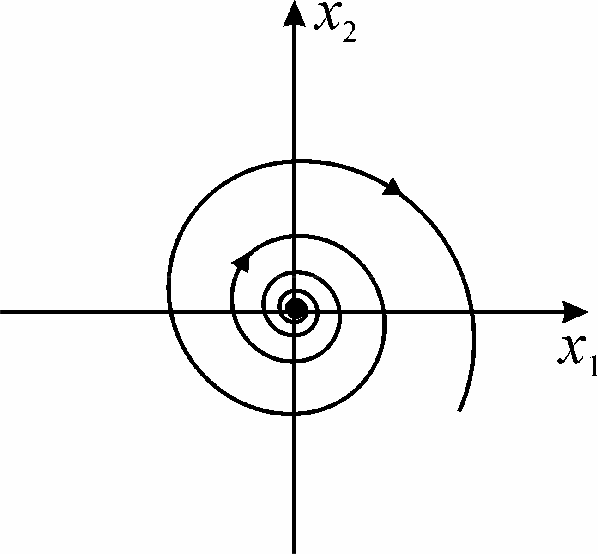
\includegraphics[width=\linewidth]{fig/lect3/7b} 
        \end{minipage}
        \begin{minipage}{0.32\linewidth}
               
\includegraphics[width=\linewidth]{fig/lect3/7c} 
        \end{minipage}                                
        \label{fig:3.7}
        \caption{Устойчивый фокус (a); неустойчивый фокус (b); центр (c).}
\end{figure}
Из первого уравнения в \eqref{eq:3.28} следует, что при $ \alpha < 0$ переменная $\rho$ монотонно убывает к нулю. Следовательно, в этом случае фазовые траектории асимптотически при $t \to \infty$ приближаются к состоянию равновесия. Такое состояние равновесия является асимптотически устойчивым и называется \textbf{ устойчивым фокусом} (рис.\ref{fig:3.7}а). Наоборот, 
если $ \alpha > 0 $ переменная $\rho$ неограниченно растёт и, следовательно, фазовые траектории удаляются от состояния равновесия (рис.\ref{fig:3.7}b).  Это состояние равновесия называется \textbf{неустойчивым фокусом}.
Заметим, что с топологической точки зрения фокус эквивалентен узлу соответствующей устойчивости, поскольку с помощью взимнооднозначного преобразования траектории одного из них могут быть переведены в траектории другого с сохранением ориентации. Несмотря на это, в многих задачах их следует различать, поскольку они определяют различные колебательные процессы. При $\alpha = 0$ переменная $\rho$ в \eqref{eq:3.27}  не меняется и, следовательно, любая нетривиальная траектории на плоскости $(u_1, u_2)$ имеет вид окружности с центром в состоянии равновесия. Такое состояние называется \textbf{центром}. На фазовой плоскости $(x_1,x_2)$ траектории могут и не совпадать с координатными осями ( рис.\ref{fig:3.7}c). Центр устойчив по Ляпунову, но не асимптотически.

\subsection{Колебания двумерных линейных систем}%
\label{ssub:3.2.3}

Как мы установили выше, разбиение фазовой плоскости на траектории
двумерных линейных систем определяются состояниями равновесия. Поэтому
возможные в таких системах колебательные процессы полностью определяется
типом состояния равновесия. Ниже в таблице \ref{tab:1} дана классификация этих
процессов и представлен их качественный вид.
\begin{table}[h!]
        \centering
        \caption{Классификация колебательных процессов}
        \label{tab:1}
        \begin{tabular}{|c|c|}
                \hline
            Состояние равновесия  & Колебательный процесс \\ \hline
            Устойчивый узел       & 
            \includegraphics[width=0.2\linewidth]{example-image-a}
            \includegraphics[width=0.2\linewidth]{example-image-a}\\ \hline
            Устойчивый фокус     & 
            \includegraphics[width=0.2\linewidth]{example-image-a}\\ \hline
            Центр                &
            \includegraphics[width=0.2\linewidth]{example-image-a} \\ \hline
            Неустойчивый узел    &
            \includegraphics[width=0.2\linewidth]{example-image-a}
            \includegraphics[width=0.2\linewidth]{example-image-a}\\ \hline
            Неустойчивый фокус   &
            \includegraphics[width=0.2\linewidth]{example-image-a} \\ \hline
        \end{tabular}
\end{table}
Принципиально другую, чем представленные в таблице состояния равновесия,
роль играет в двумерных линейных системах седло – устойчивые сепаратрисы
седла разделяют неограниченно нарастающие движения на две группы,
имеющие различное предельное поведение (см., например, рис.\ref{fig:3.5}b). 

\subsection{Двухпараметрическая буфуркационная диаграмма}%
\label{ssub:3.2.4}

Как правило, в практических задачах коэффициента $a, b ,c$ и $d$ системы
\eqref{eq:3.6} зависят от параметров, которые могут изменяться. Это изменение может вызвать смену типа состояния равновесия. Рассмотрим, как этом может произойти в случае двух параметров, которые введем следующим образом
\begin{equation}
        \label{eq:}
        \mu_1 - (a+d), \quad m_2= \det A
\end{equation}

В этих обозрачениях характеристическое уравнение \eqref{eq:3.9} перепишется в следующем виде
\begin{equation}
        \label{eq:3.30}
       \lambda^2 + \mu_1 \lambda + \mu_2 =0 
\end{equation}
\begin{figure}[h!]
        \centering
        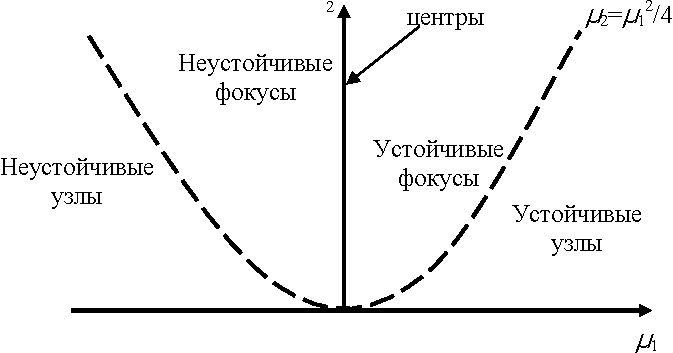
\includegraphics[width=0.8\linewidth]{fig/lect3/8}
        \label{fig:3.8}
        \caption{Разбиение плоскости $(\mu_1,\mu_2)$ на области, соответствующие различным типам состояний равновесия.}
\end{figure}
Анализируя значение корней уравнения \eqref{eq:3.30} в зависимости от параметров $\mu_1$, $\mu_2$, устанавливаем вид разбиения плоскости $( \mu_1, \mu_2)$ на области, соответствующие различным типам состояний равновесия системы \eqref{eq:3.6}. Разбиение осуществляется двумя бифурцационными прямыми --$B_1 = \{ \mu_2=0, \mu_1 \in \R \}$, $B_2=\{\mu_1=0, \mu_2>0\}$ и параболой $\{ \mu_2= \frac{\mu_1^2}{4}, \mu \neq 0 \}   $
, отделяющей узлы фокусов и не являющейся буфуркационной, поскольку эти состояния равновесия топологочески эквивалентны. На прямой $B_2$ происходит смена устойчивости фокуса черз образование центра, а на прямой $B_1$ уравнение \eqref{eq:3.30} имеет либо один, если $\mu_1 \neq 0$, либо два нулевых корня, если $\mu_1\neq 0$. иИсследуем поведение траекторий системы \eqref{eq:3.6} для точек прямой $B_1$. Сделаем в \eqref{eq:3.6} замену переменной $x_2$ :
\begin{equation}
        \label{eq:}
        y= ax_1 + bx_2,
\end{equation}
с помощью которой эта система преобразуется к виду
\begin{equation}
        \label{eq:3.31}
        \dot x_1 = y, \quad \dot y = - \mu_1 y  
\end{equation}
Из \eqref{eq:3.31} следует, что $y=0$ является линией состояний равновесия, а все остальные траектории имеют вид прямых
\begin{equation}
        \label{eq:}
        y= - \mu_1x +C, \quad C=\const
\end{equation}

Принимая во внимание эти свойства траекторий, устанавливаем портреты системы \eqref{eq:3.31} , представленные на рис.\ref{fig:3.9}.
        
\begin{figure}[h!]
        \centering
        
\includegraphics[width=0.5\linewidth]{fig/lect3/9a}
        \label{fig:3.9}
        \caption{Фазовые портреты системы \eqref{eq:3.30}  для различных значений параметра $\mu_1:$
        (a) $\mu_1>0$ ; (b) $\mu_1=0$ ; (c) $\mu_1<0$.}
\end{figure}
